%  \input{header_link}
%   \begin{document}
     		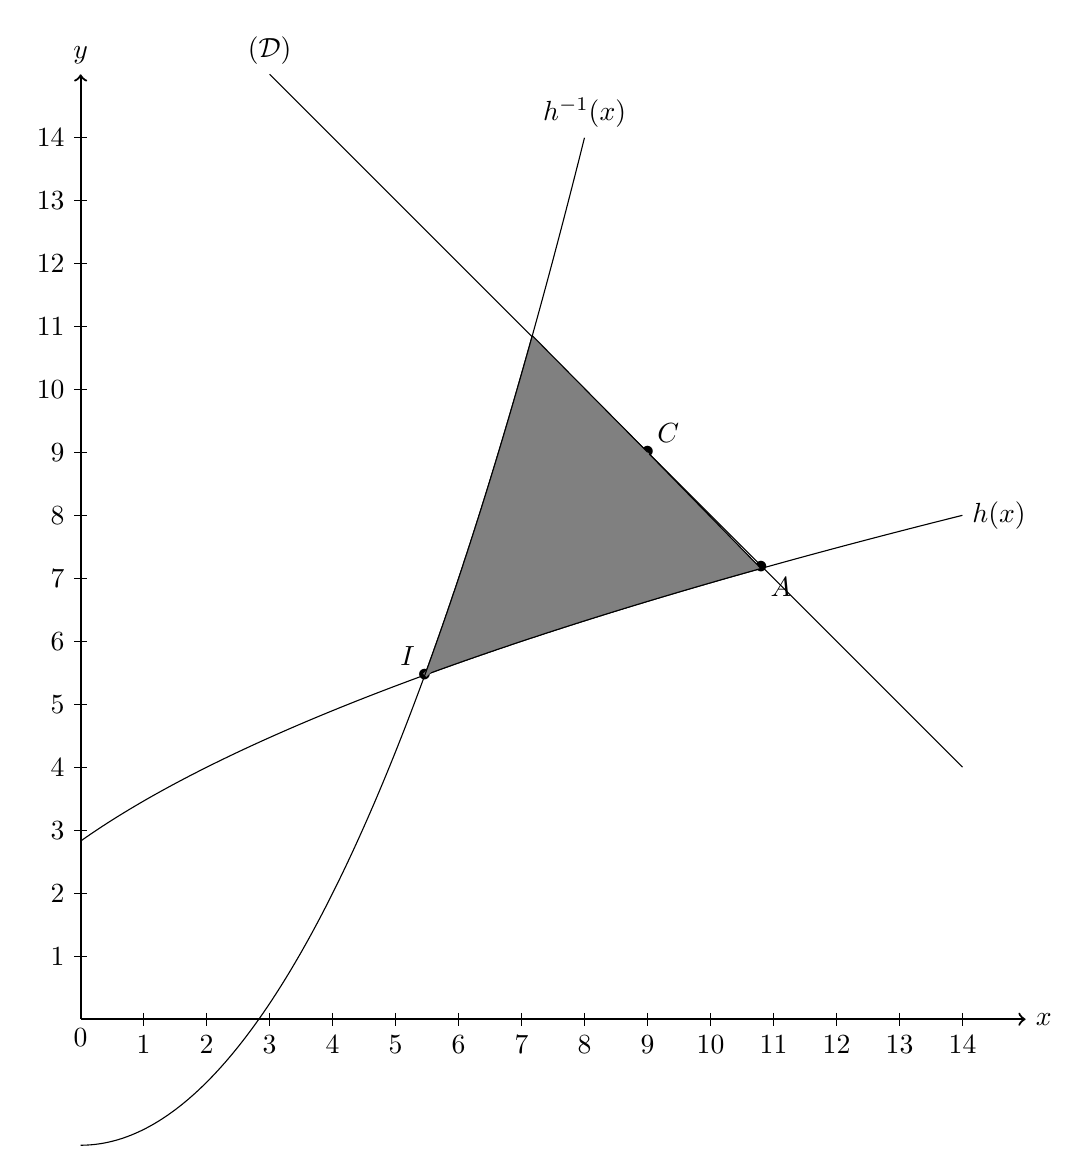
\begin{tikzpicture}[scale=0.8]
     		\draw[->,thick] (0,0)--(0,15) node[above]{$y$};
     		\draw[->,thick] (0,0)--(15,0) node[right]{$x$};
     		\foreach \x in {1,2,...,14}{
     		\draw (\x,0.1)--(\x,-0.1) node[below]{$\x $};
     		}
     		\foreach \y in {1,2,...,14}{
     		\draw (0.1,\y)--(-0.1,\y) node[left]{$\y $};
     		}
     		\node[below] at (0,0) {$0$};
     		\draw[domain=0:14,samples=200] plot({\x},{2*sqrt(\x+2)});
     		\draw[domain=3:14,samples=200] plot({\x},{-\x+18});
     		\node[above] at (3,15){$\mathcal{(D)}$};
     		\node[right] at (14,8) {$h(x)$};
     		\node at (5.46,5.46) {$\bullet$};
     		\node[above left] at (5.46,5.46) {$I$};
     		\node at (10.8,7.17) {$\bullet$};
     		\node[below right] at (10.8,7.17) {$A$};
     		\node at (9,9) {$\bullet$};
     		\node[above right] at (9,9) {$C$};
     		\node at (8,7) {\textbf{F}};
     		\draw[domain=0:8,samples=200] plot({\x},{(\x^2/4)-2});
     		\node[above] at (8,14) {$h^{-1}(x)$};
     		\draw[fill=gray] (5.46,5.46)--plot[domain=5.46:10.8]({\x},{2*sqrt(\x+2)}) -- (9,9)--cycle;
     		\draw[color=gray,ultra thick](5.46,5.46)--(9,9);
     		\draw[fill=gray] (5.46,5.46)--plot[domain=5.46:7.17]({\x},{(\x^2/4)-2}) -- (9,9);
		\end{tikzpicture}
%   \end{document}
